\documentclass[a4paper,12pt,twoside,BCOR=10mm]{scrbook}

% Packages
\usepackage[utf8]{inputenc} % Updated by Ernir
\usepackage[icelandic]{babel} % Updated by Ernir
\usepackage[T1]{fontenc} % Updated by Ernir

\usepackage{graphicx}
\usepackage[intoc]{nomencl}
\usepackage{enumerate,color}
\usepackage{url}
\usepackage[pdfborder={0 0 0}]{hyperref}
\usepackage{appendix}
\usepackage{eso-pic}
\usepackage{amsmath, amssymb} % Inlined by Ernir
\usepackage[numbib,nottoc]{tocbibind} % Numbib option added by Ernir
\usepackage[sort&compress,authoryear]{natbib}
\usepackage{subcaption} % Obsolete subfigure package removed by Ernir
\usepackage[format=plain,labelformat=simple,labelsep=colon]{caption}
\usepackage{placeins}
\usepackage{tabularx}

%%% ADDITIONS BY ERNIR
\usepackage{textcomp} % To disable font warnings http://www.latex-community.org/forum/viewtopic.php?t=8608
\usepackage{scrhack} % To suppress KOMA warning http://tex.stackexchange.com/questions/51867/koma-warning-about-toc
\usepackage{booktabs}
\usepackage[newfloat]{minted}
\usepackage[rounded]{syntax}
\usepackage{auxhook}

\SetupFloatingEnvironment{listing}{name=Kóðalistun}
\SetupFloatingEnvironment{listing}{listname=Kóðalistunarskrá}

% Custom references
\newcounter{labelknownref}
\renewcommand*{\thelabelknownref}{\the\value{labelknownref}}
\makeatletter
\AddLineBeginAux{%
  \string\providecommand\string\LabelKnown[2]{}%
}
\newcommand*{\LabelKnown}[2]{%
  \expandafter\xdef\csname lkr@#2\endcsname{%
    \@ifundefined{r@#1}{0}{1}%
  }%
}

\newcommand*{\myref}[1]{%
  \begingroup
    \stepcounter{labelknownref}%
    \if@filesw
      \protected@write\@auxout{}{%
        \string\LabelKnown{#1}{\thelabelknownref}%
      }%
    \fi 
    \if\csname lkr@\thelabelknownref\endcsname 1%
      ($\leftarrow$\ref{#1})%
    \else
      \if\csname lkr@\thelabelknownref\endcsname 0%
        (\ref{#1}$\rightarrow$)%
      \else
        (\ref{#1})%
      \fi
    \fi
  \endgroup
}
\makeatother


% Syntax diagrams
\newenvironment{repnull}[0]{%
\begin{stack}
\\
\begin{rep}
}{%
\end{rep}
\end{stack}
}
\newenvironment{syntaxenv}[1]{%
\par\noindent\begin{minipage}{\linewidth}\vspace{0.5em}\begin{quote}\noindent%
\hspace*{-2em}\synt{#1}:\hfill\par%
\noindent%
\begin{minipage}{\linewidth}\begin{syntdiag}%
}{%
\end{syntdiag}\end{minipage}\end{quote}\end{minipage}%
}
%%% END ADDITIONS



% Configurations
\graphicspath{{figs/}}

\setlength{\parskip}{\baselineskip}
\setlength{\parindent}{0cm}
\raggedbottom

% Mun fallegri lausn
\setkomafont{captionlabel}{\itshape}
\setkomafont{caption}{\itshape}
\setkomafont{section}{\FloatBarrier\Large}
% \setcapwidth[l]{\textwidth} % Ernir: Kommentað út til að þagga niður í viðvörun um að þetta hafi verið hunsað
\setcapindent{1em}

%%%%%%%%%%% MODIFY THESE LINES ONLY %%%%%%%%%%%%%%%%%%%%%%%%%%%%%%%%%%%%%%%%%%%%%%%%%%%%%%%%%
\def\thesisyear{}       						% Year thesis submitted
\def\thesismonth{}						% Month thesis submitted
\def\thesisauthor{Eiríkur Ernir Þorsteinsson}					% Thesis authoreiningaraðferðinni
\def\thesistitle{Vefkennsla í notkun gagnasafna} 						% Title of thesis
\def\thesisshorttitle{Vefkennsla í notkun gagnasafna} 	% Title of thesis
\def\thesiscredits{40} 							% Credits awarded for the project
\def\thesissubject{Menntun framhaldsskólakennara}
\def\thesiskind{M.Sc.}							% Masters of PhD thesis
\def\thesiskindformal{Magister Scientiarum}				% Masters of PhD thesis
\def\thesisnroftutors{1}						% Number of tutors
\def\thesisschool{Verkfræði- og náttúruvísindasvið}			% School
\def\thesisfaculty{Iðnaðarverkfræði-, vélaverkfræði- og tölvunarfræðideild}							% Faculty
\def\thesisaddress{Hjarðarhaga 2-6}				% Office address
\def\thesispostalcode{107 Reykjavík}			% Office address
\def\thesistelephone{699-4392}						% Office telephone
\def\thesispublisher{-}						% Publisher
\def\thesistutors{Hjálmtýr Hafsteinsson}
\def\thesisrepresentative{XXNN3}					% Tutors name
\def\thesiscommittee{XXNN4 \\ XXNN5 }
\def\thesiskeywords{SQL, Exploratory Learning}			% Keywords
\def\thesisISBN{XX}           						% Thesis ISBN number
\def\thesisdedication{Dedication}
\def\thesisPrinting{Háskólaprent, Fálkagata 2, 107 Reykjavík}

% Function to add footer to frontpage
\newcommand\BackgroundPic{
\put(0,0){
\parbox[b][\paperheight]{\paperwidth}{
\vfill
\centering
\hspace*{-0.6cm}

\includegraphics[width=\paperwidth,height=\paperheight,
keepaspectratio]{foot}
}}
\setlength{\unitlength}{\paperwidth}
\begin{picture}(0,0)(0,-0.15)
\put(0,0){\color{white}\parbox{1\paperwidth}{\centering\bfseries\sffamily \Large \thesisfaculty \\
Háskóli Íslands\\
\thesisyear}}
\end{picture}
}

\begin{document}

\hypersetup{pageanchor=false}
\begin{titlepage}
\thispagestyle{empty}
\AddToShipoutPicture*{\BackgroundPic}
%
\begin{center}
\vspace*{1cm}

\includegraphics[width=43.6mm]{logotitle}\\
\vspace*{3.0cm}
\huge \sffamily \bfseries \thesistitle

\vspace*{5.5cm}
\normalfont \Large \sffamily \thesisauthor
\AddToShipoutPicture*{\BackgroundPic}
\vfill

\end{center}

\newpage 
\thispagestyle{empty} \mbox{}
\newpage
\vspace*{1.35cm}
\thispagestyle{empty}
\begin{center}

\Large \textbf{\sffamily{\MakeUppercase{\thesistitle}}} \\

\vspace*{1.7cm}
\sffamily{\thesisauthor} \\
\vspace*{1.8cm}
\normalsize \thesiscredits~ECTS thesis submitted in partial fulfillment of a \\
\textit{\thesiskindformal} degree in \thesissubject

\vspace*{1.0cm}
\large
\ifnum\thesisnroftutors >1 Advisors \\ \thesistutors \\ \vspace*{0.4cm}
\else Advisor \\ \thesistutors \\ \vspace*{1.04cm}
\fi
Faculty Representative \\
\thesisrepresentative

\vspace*{0.4cm}
M.Sc. committee \\
\thesiscommittee

\vfill
Faculty of \thesisfaculty \\
\thesisschool \\
University of Iceland \\
Reykjavik, \thesismonth~\thesisyear
\newpage
\end{center}
 \newpage
 \thispagestyle{empty}
 \mbox{} \vfill
 % \setcounter{page}{0} \renewcommand{\baselinestretch}{1.5}\normalsize
 \sffamily{\thesistitle} \\
 \sffamily{\thesisshorttitle} \\
 \thesiscredits ~ECTS thesis submitted in partial fulfillment of a \thesiskind~degree in \thesissubject
\\ \\
Copyright \textcopyright~\thesisyear~ \thesisauthor \\
All rights reserved \\


Faculty of \thesisfaculty \\
\thesisschool \\
University of Iceland \\
\thesisaddress \\
\thesispostalcode, Reykjavik \\
Iceland

Telephone: \thesistelephone \\ \\
\vspace*{\lineskip}

Bibliographic information: \\
\thesisauthor, \thesisyear, \thesistitle, \thesiskind~thesis, Faculty of \thesisfaculty, University of Iceland. \\

ISBN~\thesisISBN

Printing: \thesisPrinting \\
Reykjavik, Iceland, \thesismonth~\thesisyear \\
% \newpage
% \thispagestyle{empty} \mbox{}
% \vfill
% \begin{center}\textit{\thesisdedication}\end{center} \vspace*{5cm}
% \vfill 

\thispagestyle{empty}
\cleardoublepage
\end{titlepage}
\hypersetup{pageanchor=true}

% \dedication{\textit{Dedication} \small \\ Tileinkun má sleppa og skal þá fjarlægja blaðsíðuna. \\
% Tileinkun skal birtast á oddatölu blaðsíðu (hægri síðu).}
\pagenumbering{roman}

\setcounter{page}{5}
\section*{\huge Abstract}
Útdráttur á ensku sem er að hámarki 250 orð.
\vfill \vspace*{1cm}
\section*{\huge Útdráttur}
Hér kemur útdráttur á íslensku sem er að hámarki 250 orð. Reynið að koma útdráttum á eina blaðsíðu en ef tvær blaðsíður eru nauðsynlegar á seinni blaðsíða útdráttar að hefjast á oddatölusíðu (hægri síðu).
\vfill
\newpage

\tableofcontents
\listoffigures
\listoftables
\listoflistings

% \chapter*{Acknowledgments}
% \addcontentsline{toc}{chapter}{Acknowledgments}
% 
% Hjálmtýr Hafsteinsson
% 
% Hrefna Karítas Sigurjónsdóttir

\chapter{Inngangur}

\pagenumbering{arabic}
\setcounter{page}{1}

\section{Forsaga verkefnisins}
Sumarið 2014 skrifaði höfundur stutta kennslubók, til stuðnings við kennslu í fyrstu áföngum Tækniskólans í Reykjavík í notkun gagnasafna. Lagst var í skrifin eftir að ljóst var að nálgun nýlegra íslenskra bóka um gagnasafnsfræði\cite{sigurdur2003, jon2008} hentaði illa fyrir 16 til 17 ára nemendur.

Þarfir áfanganna í Tækniskólanum eins og þeir voru kenndir á þeim tíma voru í forgrunni við skrif bókarinnar. Farið var hægt yfir grundvallaratriði fyrirspurna og annarra mikið notaðra atriða í MySQL gagnagrunnskerfinu.

Kennslubókin var, með styrk frá Þróunarsjóði námsgagna, gefin út rafrænt sem PDF-skjal. Bókin var og er öllum aðgengileg á Github-síðu höfundar\footnote{\url{https://github.com/Ernir/sql-bok-ts}}. 

Bókinni var vel tekið af þeim kennurum Tækniskólans sem sáu um kennslu í notkun gagnasafna. Engu að síður varð fljótt ljóst að efninu mætti betur koma til skila með öðrum hætti - í gegnum vafrann.
\section{Önnur kennslutól}
Hugmyndin um að nýta vefinn og tölvuforrit til kennslu í notkun gagnasafna er ekki ný af nálinni. Auðvelt er að finna umfjöllun um eldri kennsluforrit sem upprunin eru í akademísku umhverfi. Auk þess hefur verið gríðarmikil gróska í gerð ýmissa veftóla til SQL-kennslu sem búin hafa verið til utan háskólaumhverfis. Verður nokkrum þeirra lýst hér að neðan.

\subsection{Akademísk SQL-kennslutól}
SQL-Tutor \cite{mitrovic1998} er kerfi komið til ára sinna, en þróun á því hófst árið 1996. Kerfið er, ætlað til að uppfylla hlutverk leiðbeinanda þegar nemandi vinnur að því að semja fyrirspurnir. Kerfið tekur við fyrirspurnum frá nemendum og metur hvort þær séu réttar, en í stað hefðbundinna villuskilaboða leggur SQL-Tutor áherslu á að veita nemandanum leiðsögn um hvað það er sem gæti hafa farið úrskeiðis. Á sínum tíma vakti það athygli fyrir notkun á ``Constraint Based Modelling'' (CBM) í stað þess að notast við villubanka. Nýrri útgáfur kerfisins eru enn að einhverju leyti virkir og notaðir til rannsókna. Sem elsta kerfið sem enn er í notkun hefur það fengið nokkra viðurkenningu sem brautryðjandi \cite{mitrovic2016implementing}.

Acharya\cite{bhagat2002} er svipaðs eðlis, en það er ITS-kerfi sem líka leggur áherslu á greiningu nemendafyrirspurna. Acharya leyfir frjálsa könnun nemandans á efnisatriðum og sýnir honum ráðleggingar byggðar á þeim efnisatriðum sem hann hefur þegar skoðað, en aðferðunum sem notaðar eru til að framleiða ráðleggingarnar er einungis lýst stuttlega. Acharya er ekki 

AsseSQL \cite{prior2014assesql} er tól til að veita sjálfvirka endurgjöf og ákvarða einkunnir. SQLator \cite{sadiq2004sqlator} leyfir nemendum að kanna gagnagrunn fyrirspurna til að framkvæma og fá endurgjöf á æfingum.

\subsubsection{Greining}
Akademísku kerfin bera þess merki að vera að mestu leyti unnin af einstaklingum. Kerfin eru skrifuð af akademískum starfsmönnum til eigin nota. Þau eru notuð við kennslu í námskeiðum sem höfundurinn kennir sjálfur og við kennslutengdar rannsóknir.

Athygli vekur að öll kerfin leggja áherslu á að greina fyrirspurnir, sum með afar sérhæfðum aðferðum. SQL-Tutor notar áðurnefnt CBM, Acharya notar sanntöflur og leggur sérstaka áherslu á að greina \texttt{WHERE} klausur.

Kerfin gera ráð fyrir að þau séu notuð sem æfingakerfi hefðbundinnar kennslu til stuðnings. Þau innihalda ekki allar upplýsingar sem nemandi þarf til að leysa verkefnin, ekkert kerfanna hefur það sem yfirlýst markmið að koma í stað fyrirlestra eða kennslubókar. 

Hið versta sem akademísku kerfin eiga sameiginlegt er þó að vera almenningi ekki aðgengileg. Höfundur hefur ekki fengið tækifæri til að keyra eitt einasta þeirra á eigin vél. Vefútgáfa SQL-Tutor, SQLT-Web, var á tímabili aðgengileg og fjölsótt á mælikvarða þess tíma\cite{mitrovic2003intelligent}, en í dag er hún eingöngu aðgengileg í viðkomandi háskóla. Lærdómurinn sem af þeim má draga er því einskorðaður við þá umfjöllun sem höfundar skilja eftir sig, ekki er hægt að læra af upplýsingunum sem felast í forritskóða kerfanna, uppsetningu þeirra eða gögnum.

\begin{figure}
\caption{Vefútgáfa SQL-Tutor\cite{mitrovic2016sqltutorweb}}
\label{fig:sqltutorweb}
\begin{center}
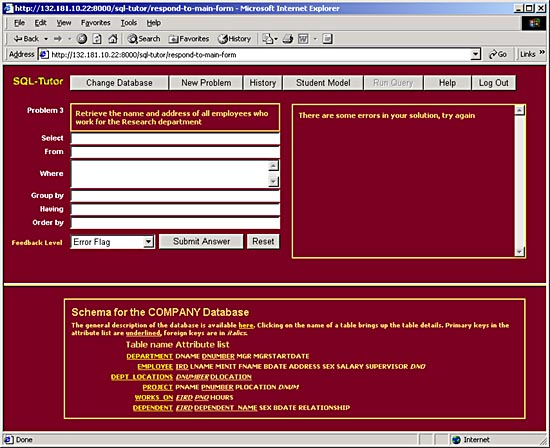
\includegraphics[width=0.8\textwidth]{sqlt-web}
\end{center}
\end{figure}

\subsection{Önnur SQL-kennslutól}
\label{sec:other-sql-teaching-tools}
Khan Academy er bandarísk menntastofnun sem ekki er rekin í gróðaskyni. Stofnunin hefur vakið athygli fyrir kennslu byggða á myndböndum, en hún býður meðal annars upp á stutta yfirferð á SQL með SQLite\footnote{\url{https://www.khanacademy.org/computing/computer-programming/sql}}. Auk myndbandanna býður SQL-námskeið Khan Academy nemendum upp á að keyra SQL-skipanir í vafraglugga sínum, á sama sniði og er notað í fyrirlestramyndböndunum. Nemandanum er umbunað með stigum fyrir framgang sinn í myndbandaáhorfi og æfingum. Nemandinn er leiddur með fastmótuðum hætti í gegnum námsefnið - þó að nemandinn geti stjórnað hraða sínum sjálfur eru ekki mikil tækifæri til sjálfstæðrar könnunar. Uppbygging efnisins er miðuð að sjálfsnámi nemenda, þeir hlutar kerfisins sem snúa að kennurum og samskiptum þeirra við nemendur eru seinni tíma viðbætur.

Kerfi sem hefur verið notað til stuðnings í Tækniskólanum er SQLZoo\footnote{\url{http://sqlzoo.net/}}. Um ``interactive tutorial'' er að ræða, þar sem nemandanum gefst kostur á að vinna sig í gegnum sífellt flóknari verkefni. Hægt er að framkvæma SQL-skipanir á vefsíðunni sjálfri, með tafarlausri endurgjöf. Síðan er byggð á MediaWiki og hún þar með opin fyrir breytingum utanaðkomandi aðila.
Líkt og í mörgum öðrum kennslukerfum samanstendur SQLZoo fyrst og fremst af æfingum í að framkvæma fyrirspurnir. Upplýsingum er ekki gefið samhengi, heldur er nemandanum strax beint að því að fara að skrifa SQL-skipanir. Framvindan í gegnum námsefnið er fyrst og fremst línuleg.

Schemaverse\footnote{\url{https://schemaverse.com/}} er leikur fremur en kennslutól, en leikurinn er spilaður með því að framkvæma SQL-skipanir til að stjórna ``geimskipum'' sem keppa við geimskip annarra. Möguleiki er á að nota leikinn til þjálfunar fyrir lengra komna nemendur og þá sem hvattir eru af samkeppni.

Nemendur sem vilja sækja formlegra netnámskeið hafa úr mörgu að velja. Coursera\footnote{\url{https://www.coursera.org/}} og edX\footnote{\url{https://www.edx.org/}} bjóða bæði upp á fjölmörg námskeið sem tengjast gagnagrunnum.

\subsubsection{Greining}
Óakademísku tólin mynda fjölbreyttari hóp en þau akademísku. Sum eru hluti af breiðu námsúrvali ósérhæfðari menntastofnunar (Khan Academy), önnur bera þess merki að vera búin til af einstaklingum eða fámennum hópi í gróðaskyni (SQLZoo) og önnur jafnvel sem áhugamál (Schemaverse).

Framsetning er í sumum tilfellum gríðarlega markviss, eins og við má búast af kerfum sem ekki geta gengið að nemendahóp vísum. Stærri síðurnar (Coursera, edX, Khan Academy) eru nútímalegar og vel hannaðar, SQLZoo er með áberandi stutta leið frá forsíðu að SQL-æfingum. Munurinn er sérlega sláandi þegar þau eru borin saman við akademísku tólin sem eru ekki einu sinni aðgengileg á netinu og bera þess vott að njóta ekki reglulegra viðmótsuppfærslna, sjá \myref{fig:sqltutorweb}.

Endurgjöf er jákvæð - Khan Academy gefur stig, SQLZoo gefur glaðlega broskalla þegar æfingu er lokið. Verið er að búa til hvata fyrir nemendur til að halda áfram þegar ytri þrýstingur (á borð við hættuna á að falla í námskeiði) er ekki endilega til staðar.

Opnu tólin þjást að mati höfundar helst af annars vegar stefnuleysi og hins vegar skorti á möguleikum til að þætta tólið saman við hefðbundna kennslu. Tólin þurfa að geta þjónað mjög breiðum hópi nemenda til að viðhalda vinsældum sínum, sem takmarkar þau í að bjóða upp á sérhæft efni. Tólin eru miðuð að nemendum sem stunda sjálfsnám, kennarar sem hyggjast nýta þau í kennslustofu þurfa að nota óbeinar aðferðir til að fylgjast með og taka þátt í framgangi nemenda.

Af velgengni þeirra má læra, en kennsluvefur sem hefur það sérstaka hlutverk að styðja við kennslu í hefðbundnu námskeiði þarf að hafa aðrar áherslur.
\chapter{Hugmyndafræði}
Yfirlit þess sem ég ætla að gera betur/á annan hátt.
\section{Vefurinn sem bók}
\label{sec:web-as-book}
Forveri verkefnisins er kennslubók. Bókin var gefin út rafrænt, en nýtti sér þá kosti sem slíkt fyrirkomulag hefur í för með sér ekki nema að takmörkuðu leyti. Innri og ytri tenglar voru til staðar í bókinni, en að flestu öðru leyti var um nokkuð hefðbundið rafrænt skjal að ræða.

Kennsluvefurinn er hugsaður sem ítrun, eða næsta útgáfa, á rafrænu kennslubókinni. Ekki er um að ræða endurskrift frá grunni, heldur er ætlunin að endurnýta það sem gefist hefur vel og bæta við virkni sem ekki var mögulegt að útfæra sem hluta af .pdf skjalinu. 

Nálgunin er því með öðrum hætti en á öðrum SQL-kennslusíðum, t.d. SQLZoo eða Khan Academy \myref{sec:other-sql-teaching-tools}, þar sem nemandanum er annars vegar beint í átt að æfingaverkefnum og hins vegar í átt að kennslumyndböndum. Áhersla kennsluvefsins er sem sagt eftir sem áður á framsetningu á ``gamaldags'' efnistexta.

Venjulegur texti hefur ýmsa kosti í för með sér. Þeir sem voru höfundi efst í huga eru þó umfram allt þrír:

\begin{itemize}
 \item Aukinn möguleiki á að nýta eldra efni, sjá vefinn sem ítrun á eldri útgáfu hér að ofan
 \item Auðveldari uppfærslur, sjá endingargildi \myref{sec:durability}
 \item Auðveldari samþætting efnis frá öðrum höfundum, sjá opið efni \myref{sec:open-material}
\end{itemize}

Þekktasta dæmið um síðu sem hefur verið unnin með þessum hætti er Wikipedia\footnote{\url{https://www.wikipedia.org/}}, sem vart þarfnast kynningar. Sú síða hóf göngu sína sem ítrun á hugmyndinni um alfræðiorðabók og ber hún þess merki. Aðalefni síðunnar er enn á textasniði með myndbönd og hljóðefni eru í aukahlutverki og framsetning efnisins er með aðskildum greinum sem vísa hver í aðra. 

Þó að áhersla sé á að varðveita nokkur af betri einkennum kennslubóka eru tvö atriði sem sérstaklega var lagt upp með að bæta við. Þau eru gagnvirkar æfingar \myref{sec:exercise-explanation} og ólínuleg framvinda \myref{sec:nonlinearity}.


% Texti frekar en vídeó af því texta er auðvelt að uppfæra.
\section{Endingargildi}
\label{sec:durability}
Kerfi byrja að úreldast um leið og þau eru gefin út. Án stöðugs viðhalds höfunda brotna þau niður og hverfa, breytast í sögudæmi. Slík viðhaldsvinna er erfið og dæmin\cite{bhagat2002, mitrovic2003intelligent, sadiq2004sqlator} sanna að ekki er hægt að reiða sig á að hún haldi áfram eftir áratug.

Til að sporna við eðlilegri hnignun þessa kennsluvefs eftir að höfundur mun óumflýjanlega hverfa til annarra starfa er leitað í hugmyndasmiðju opins hugbúnaðar (e. \emph{open source software}). Kennsluvefurinn er opinn á þrenna vegu - kennsluefni vefsins er opið, grunnkóði vefsins er opinn og allur hugbúnaður sem vefurinn byggir á er líka opinn.
\subsection{Opinn kóði}
\label{sec:open-source}
Allur grunnkóði vefsins er opinn og aðgengilegur á Github-síðu höfundar\footnote{\url{https://github.com/Ernir/sql-web}}. Hver sem er getur skoðað kóðann og sett hann upp á sinni vél og breytt honum að vild, í samræmi við skilmála opins kóðaleyfis \myref{code:license} sem dreift er með kóðanum. Kóðanum er dreift með Git\footnote{\url{https://git-scm.com/}} útgáfustjórnunarkerfinu, sem er sérstaklega hannað til að virka án miðlægs vefþjóns. Endingargildi kerfisins er þar með aukið umfram það sem höfundur gæti boðið upp á - kerfið mun lifa svo lengi sem einhver sem sótt hefur kóðann heldur honum aðgengilegum og uppfærslur munu geta borist svo lengi sem kerfið er í notkun.

Það að hver sem er geti sett upp keyrandi útgáfu af kennsluvefnum myndar líka hornsteininn í dreifingarmöguleikum kerfisins. Vefurinn er ekki takmarkaður við eina, skilgreinda útgáfu sem stjórnað er af höfundi, heldur getur hver skóli eða jafnvel hver áfangi, keyrt sína eigin sérsniðnu útgáfu. Til dæmis gefur þetta möguleika á að sérsníða afkastagetu vefsins, skóli með smáar þarfir getur notast við einfalda, ódýra vefhýsingu en stærri skóli gæti tileinkað vefnum heilan vefþjón.

Höfundur hyggst halda úti grunnútgáfu af vefnum sem verður aðgengilegur á léni í eigin eigu. En fari svo að höfundur hverfi frá verkefninu og sú útgáfa sem á því léni verði aftend er vefurinn sjálfur þar með ekki dauður og gleymdur - allar aðrar útgáfur munu áfram virka og grunnkóðinn verður enn til.
\subsection{Opinn hugbúnaður í notkun}
Allar tæknilausnir sem vefurinn notar eru opnar og ókeypis, líkt og kóði vefsins sjálfs. Um tæknilausnir má lesa nánar í \myref{sec:third-party-tech}.

Það að hver sem er geti sett upp keyrandi útgáfu af kennsluvefnum er því ekki takmörkuð við þá notendur sem hafa aðgang að sérstökum, lokuðum hugbúnaði.

Eitt og sér tryggir það að tæknilausnirnar séu opnar ekki langlífi þeirra, frekar en það að kóði kennsluvefsins sé opinn tryggir það fyrir vefinn sjálfan. 
En fyrirkomulagið gerir það að ein tiltekin lausn sem kennsluvefurinn reiðir sig á verði skyndilega óaðgengileg mun ólíklegri.
\subsection{Opið efni}
\label{sec:open-material}
Kóðanum og efninu sem vefurinn inniheldur er dreift samhliða og með svipuðum aðferðum. 
Meðal afleiðinga þess er að allt efni vefsins breytanlegt af notendum hans, í samræmi við skilmála opins efnisleyfis \myref{code:license}. Sérstakar viðbætur \myref{sec:markdown-additions} voru gerðar til að gera efnissmíði við hæfi kennsluvefsins auðveldari.

Hver kennari getur þannig bætt við ``köflum'' í bókina, falið hluta efnisins og framkvæmt hverjar þær áherslu- og efnisbreytingar sem viðkomandi þóknast.
Þetta mætti til dæmis nota til að bæta við stuðningi við nýtt gagnagrunnskerfi eða til þess að fella sérsniðin myndbönd inn í textann.

Fyrirkomulagið hefur sömu afleiðingar fyrir endingargildi efnisins og opna kóðafyrirkomulagið hefur fyrir endingargildi vefsins sjálfs.
\section{Viðfangsefni sem net/Topic Maps}
\section{Myndræn framsetning}
\section{Ólínuleg framvinda}
\label{sec:nonlinearity}
\section{Efnisáherslur}
\subsection{Æfingar}
\label{sec:exercise-explanation}
\chapter{Útfærsla vefsins}
% Vefurinn er skrifaður í forritunarmálinu Python með notkun Django \myref{sec:django}. Efnið er skrifað með Markdown \myref{sec:markdown}.


\section{Tæknilausnir frá þriðja aðila í notkun}
\label{sec:third-party-tech}
\subsection{Django}
\label{sec:django}
Django er vefburðargrind (e. \emph{web framework}) fyrir Python-forritunarmálið. Slík burðargrind veitir meiri stuðning en bein Python-forritun gegn vefþjóni, en mun minni stuðning en vefumsjónarkerfi eins og WordPress. Django var fyrst gefið út árið 2005 af Adrian Holovaty og Simon Willison, sem þróuðu kerfið út frá forritum sem þeir höfðu notað við netblaðaútgáfu. Það er mest notaða Python vefburðargrindin í dag.

Django fylgir Model-View-Controller (MVC) hönnunarmynstrinu eins og það er venjulega túlkað á vefnum. Flest ``fyrirbrigði'' kennsluvefsins eru þannig skilgreind af Python-forritsklösum sem tengjast Object-relational Mapping (ORM) kerfi grindarinnar \myref{sec:django-orm}.

Burðargrindin hjálpar einnig stórlega við kóðaendurnýtingu og framsetningu. Sem dæmi má taka að stílsupplýsingar sem eru öllum undirsíðum kennsluvefsins sameiginlegar má finna í einni grunnskrá \myref{code:base-template}.
\subsubsection{Django ORM}
\label{sec:django-orm}
Object-relational Mapping kerfi Django heldur utan um gagnagrunnstengingar og upplýsingar sem viðkoma Django-vefsíðu.

Kerfið er hlutbundið. Klasi sem táknar ``fyrirbrigði'' í Django erfir frá \texttt{model} klasa gefnum af burðargrindinni. Forritarinn bætir síðan við eigin eiginleikum og aðferðum sem viðkoma forritinu. Burðargrindin sér um að smíða gagnagrunnstöflur sem geymt geta þær upplýsingar sem þarf til að tákna tilvik af klasanum.

Vensl á milli fyrirbrigða skilgreinast líka af ORM-kerfinu. Þannig er hugtakið \texttt{Section} t.d. tengt við hugtakið \texttt{Excercise} með eiginleikanum \texttt{associated_exercises} sem skilgreindur er í \texttt{Section} klasanum og vísar á \texttt{Exercise} klasann með nafni, sjá kóðalistun \myref{code:orm-example}. Allir \texttt{model} klasar sem viðkoma kennsluvefnum eru skilgreindir í skránni \texttt{sql\_web/models.py} \myref{code:django-model-objects}.

\begin{listing}
\caption{Hluti Section klasans, vensl milli ``Section'' og ``Exercise'' skilgreind}
\label{code:orm-example}
\begin{minted}[frame=lines]{python}
class Section(models.Model):
    """..."""
    associated_exercises = models.ManyToManyField("Exercise")
    """..."""
\end{minted}

\end{listing}


\subsection{Markdown}
\label{sec:markdown}
Greinar kennsluvefsins eru skrifaðar í ívafsmálinu (e. \emph{markup language}) Markdown\footnote{\url{http://daringfireball.net/projects/markdown/}}. Markdown er mikið notað, líklegt er að kennarar í tölvugreinum hafi rekist á afbrigði af Markdown á síðunum Github\footnote{\url{https://github.com/}}, Stack Overflow\footnote{\url{http://stackoverflow.com/}} eða á spjallborði á netinu.

Aðaláhersluatriði Markdown er að frumkóði (e. \emph{source code}) textaskjalsins sé læsilegur og auðskrifanlegur. Þetta er ólíkt þekktasta ívafsmálinu, HTML, þar sem markmiðið er að skilgreina einingar til framsetningar. HTML inniheldur þess vegna töluverðar viðbótarupplýsingar um hvernig birta skal textann, sbr. mynd \myref{fig:markdown} sem eru áskildar í Markdown.

\begin{figure}
\caption{Upprunalegur Markdown-kóði og HTML-ið sem hann skilgreinir}
\label{fig:markdown}
\begin{center}
\texttt{Markdown styður *skáletrun*}

$\downarrow$

\texttt{<p>Markdown styður <em>skáletrun</em></p>}

\end{center}
\end{figure}

Markdown-sniðið er sem sagt sérstaklega hannað til að skrifa texta án truflana, sem svo er oft þýddur yfir í þyngri ívafsmál (venjulega HTML) með þar til gerðu forriti. Markdown-málið er upphaflega skilgreint óformlega með slíku forriti, Perl-forritinu \texttt{Markdown.pl}, skrifað af John Gruber árið 2004. Kennsluvefurinn notar Markdown á svipaðan hátt, tekið er við Markdown-texta frá efnishöfundi og hann þýddur yfir á HTML með Markdown-túlki. Útfærslan sem kennsluvefurinn notar er Markdown-pakki Python forritunarmálsins\footnote{\url{https://pypi.python.org/pypi/Markdown}}.

Sérstakar viðbætur voru gerðar við Markdown-pakkann til að styðja sérkröfur kennslufvefsins \myref{sec:markdown-additions}.
\subsection{D3.js}
\subsection{Tufte-css}
\label{sec:tufte-css}
\section{Sérsmíðaðar tæknilausnir}
\subsection{Greining á SQL-skipunum nemenda}
\label{sec:command-analysis}
Ólíkt fyrri kennslutólum sem leggja mikla áherslu á að greina nemendafyrirspurnir\cite{mitrovic1998, bhagat2002} leggur kennsluvefurinn áherslu á framsetningu efnisins. Í samræmi við þá áherslu eru þau tól sem vefurinn notar til að greina fyrirspurnirnar einföld.

Til að keyra SQL-skipun þarf nemandinn að leysa svokallaða æfingu. Æfing (e. \emph{exercise}) í kennsluvefnum er skilgreind af Django \myref{sec:django} \texttt{model} hlut, sjá \texttt{Exercise} klasann \myref{code:django-model-objects}. Slíkur hlutur hefur nokkra eiginleika sem vert er að nefna:

\begin{itemize}
 \item Nafn, auðkenni og lýsingu
 \item Gerðarlýsingu (e. \emph{schema}) ásamt gögnum, sem sett er upp áður en skipanir eru keyrðar
 \item SQL-skipun sem ætlunin er að láta nemandann líkja eftir
 \item Sjálfgefna skipun, sem nemandinn skal breyta
 \item Tilgreiningu á ``gerð'' æfingarinnar - \texttt{SELECT} æfing eða annars konar æfing
\end{itemize}

Þessir eiginleikar, að viðbættri SQL-skipun sem nemandinn skrifar inn, mynda eina keyrslu á æfingu. Keyrsla á æfingu skilar sanngildi sem tilgreinir hvort SQL-skipun nemandans hafi verið rétt miðað við gefnar forsendur, ásamt skilaboðum til nemandans.

Keyrsla er framkvæmd í skránni \texttt{sql\_web/sql\_runner.py} \myref{code:example-runner}. Hún fer fram í nokkrum skrefum. Ávallt eru grundvallar-athuganir gerðar á inntaki notandans, athugað er hvort að breytingar hafi verið gerðar á sjálfgefnu skipuninni og hvort einhver skipun hafi verið slegin inn yfir höfuð. Önnur skref eru mismunandi eftir því hvort að um \texttt{SELECT}-skipun sé að ræða eða ekki.

\subsubsection{Mat á SELECT skipunum}
Þegar um \texttt{SELECT}-skipanir er að ræða er möguleiki á að sannreyna niðurstöðurnar á sveigjanlegri máta.

Í slíkum æfingum er gerðarlýsingin sett upp og fyrirspurnirnar, bæði fyrirspurn nemandans og samanburðarfyrirspurnin, keyrðar á henni. Út úr þeim keyrslum koma tvö mengi niðurstaðna sem hægt er að bera saman, annars vegar ``nemendamengi'' og hins vegar ``samanburðarmengi''. Séu mengin eins er nemendaskipunin talin rétt.

Gagnagrunnsviðmótið skilar niðurstöðumengjunum sem listum (e. \emph{lists}) af línum (e. \emph{tuples}). Þessar gagnagrindur (e. \emph{data structures}) eru almenns eðlis, sem setja möguleikum á samanburðum nokkrar skorður.

Samanburðurinn fer fram með eftirfarandi hætti:
\begin{itemize}
 \item Athugað er hvort að mengin séu af sömu stærð, séu þau það ekki er samanburðinum strax hafnað
 \item Ítrað er yfir samanburðarmengið og leitað að tilsvarandi stökum í nemendamenginu
 \begin{itemize}
  \item Stökin eru fjarlægð úr tilsvarandi mengjum við samanburðinn
  \item Keyrslu er hætt finnist stak ekki í nemendamenginu
  \item Sé samanburðarmengið myndað með fyrirspurn sem inniheldur \texttt{ORDER BY} er sú krafa gerð að stakið sé fremst í nemendamenginu
 \end{itemize}
 \item Samanburðurinn á milli mengjanna er sannur ef ítrunin tæmir þau bæði.
\end{itemize}

\begin{table}
\caption[Tímaflækja samanburða]{Tímaflækja samanburða á fyrirspurnamengjum í æfingum kennsluvefsins}
\label{tab:comparison-complexity}
\begin{center}
\begin{tabular}{ll}
\toprule
Aðgerð&Tímaflækja í versta tilfelli\\
\midrule
Staðfesting á misstórum mengjum& $O(1)$\\
Samanburður á óröðuðum mengjum& $O(n^2)$\\
Samanburður á röðuðum mengjum& $O(n)$\\
\bottomrule
\end{tabular}
\end{center}
\end{table}
Ítrunin yfir samanburðarmengið tekur línulegan tíma með tilliti til fjölda staka í menginu. Einföld samanburðarleit á borð við þá sem notuð er á nemendamengið er sömuleiðis með línulegan keyrslutíma. Gert er ráð fyrir því að samanburður tveggja lína taki fastan tíma.

Áætlaðar tímaflækjur fyrir samanburði niðurstaðnanna má sjá á töflu \myref{tab:comparison-complexity}. Nokkur tímasparnaður næst fram á röðuðum mengjum, þar sem ekki þarf að renna í gegnum allt nemendamengið á hverri ítrun yfir samanburðarmengið. Tímaflækja samanburðanna er slæm þegar bera þarf saman tvö óröðuð, jafn stór mengi. Þetta hefur engu að síður ekki valdið vandræðum við raunverulegar aðstæður. Aðferðin hefur auk þess nokkra kosti sem gera hana áreiðanlegri en fyrirsjáanlegir möguleikar á að nota skilvirkari aðferðir.

\paragraph{Aðrar leiðir til að framkvæma samanburði} Þekkt er að hægt sé að bera saman tvö mengi á línulegum tíma með tilliti til fjölda staka sé uppfletting möguleg á föstum tíma. Mengi í Python styðja uppflettingu á föstum tíma, að því gefnu að hægt sé að reikna tætivistföng (e. \emph{hash values}) fyrir stökin. Þar sem kennari getur útbúið æfingar með flestum gerðum gagna er óáreiðanlegt að gera ráð fyrir miklu um uppbyggingu hverrar línu.

Einnig er hægt að bera saman mengi á $O(n\log n)$ tíma séu stökin raðanleg. Hvoru mengi um sig er þá raðað með samanburðarröðunarreikniriti og stök mengjanna þvínæst pöruð saman í röð. Þessi leið er einnig illfær. Þó að gögn í gagnagrunnum séu jafnan þess eðlis að hægt sé að raða þeim, þá er röðun ekki áreiðanleg nema á þau sé skilgreindur lykil. Ekki er hægt að stjórna sniði nemendafyrirspurnarinnar, svo ákvörðun á lykli fyrir þær fyrirspurnir væri líka óáreiðanleg.

Báðar leiðinar eru skilvirkari en sú sem valin er, en fela í sér möguleikann á ólíklegum en torskildum villum fyrir notendur vefsins.
\subsubsection{SQLite í minni}
Allar SQL-skipanir nemenda sem kennsluvefurinn keyrir eru keyrðar á SQLite gagnagrunni sem einungis er til í minni kerfisins. Þegar meta skal skipun er tómur gagnagrunnur búinn til í minni, gerðarlýsingin sett upp, nemendafyrirspurnin og samanburðarfyrirspurnin keyrð og gagnagrunninum að lokum eytt. Sjá mynd \myref{fig:sql-evaluation-execution}.	

\begin{figure}
\caption{Framkvæmd mats á nemendafyrirspurn}
\label{fig:sql-evaluation-execution}
\begin{center}
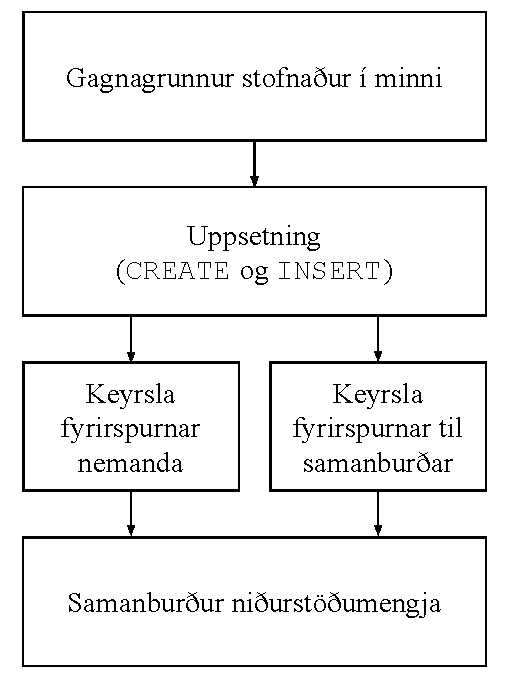
\includegraphics{KeyrslaFyrirspurnar}
\end{center}
\end{figure}

Helsti kostur þessa fyrirkomulags er öryggi. Gagnagrunnurinn er tímabundinn og inniheldur engin gögn nema þau sem eru æfingunni viðkomandi. Tengingin hefur ekki heimildir til að tengjast skráarkerfinu né heldur til að framkvæma SQLite-stýriskipanir (``dot-commands'') sem gætu framkallað breytingar á kerfinu sjálfu eða lesið þaðan upplýsingar. Það er aldrei hættulaust að keyra kóða annars fólks með jafn litlu eftirliti og forritunarkennslukerfi krefst, en með þessum hætti er tekið fyrir algengustu gerðir skaðlegra villna og árása.

Skortur á keyrsluhraða hefur ekki valdið vandræðum með þessu fyrirkomulagi. Þó að það að stofna til nýs gagnagrunns í hvert skipti sem nemandi framkvæmir fyrirspurn feli í sér tímakostnað hefur hann ekki verið greinanlegur. Líklegt er að það að gagnagrunnur í minni krefjist ekki diskaðgangs vegi á móti, auk þess sem gagnasöfnin sem um ræðir eru af viðráðanlegri stærð, verandi af stærð sem nemendur geta meðtekið.
\subsubsection{Mat á skipunum öðrum en SELECT skipunum}
Snúist æfingin ekki um \texttt{SELECT} skipun er strengjasamanburður notaður til að athuga hvort að skipunin sé sambærileg við þá sem herma skal eftir. Samanburðurinn felst í því að Levenshtein-fjarlægð er reiknuð á milli skipananna tveggja. 

Levenshtein-fjarlægð er mælikvarði á hversu líkar tvær runur eru. Í þessu tilviki er um að ræða talningu á því hversu margar eins stafs breytingar þyrfti að gera á streng sem inniheldur fyrirspurn nemandans til að breyta henni í fyrirspurn kennarans.

Fjarlægðin er reiknuð án þess að taka tillit til biltákna (e. \emph{whitespace characters}) eða mismunar á milli hástafa og lágstafa. Sé Levenshtein-fjarlægðin á milli strengjanna 0 er skipunin rétt, annars röng. Sé skipunin röng og fjarlægðin lítil er nemandanum birt fjarlægðin, ásamt útskýringu. Markmiðið með að birta Levenshtein-fjarlægðina sé hún lág er til að gefa nemendum vísbendingu um að viðkomandi gæti verið á réttri leið en með smávægilega málskipunarvillu (e. \emph{syntax error}), en málskipunarvillur er sá villuflokkur sem nemendur lenda hvað oftast í við að skrifa SQL\cite{ahadi2016students}.

\subsection{Markdown viðbætur}
\label{sec:markdown-additions}
Markdown er einfalt mál og er þar af leiðandi með fáa sérhæfða möguleika tengdum framsetningu textans. Auk þess eru Markdown-túlkar einfeldningsleg textatúlkunarforrit, sem ekki gera sér grein fyrir innri uppbyggingu texta eða tengsla á milli viðfangsefna. Til að styðja myndræna framsetningu og innri tengingar textans er því nauðsynlegt að smíða viðbætur við túlkinn.
 
Opinbera viðbótin \texttt{tables} við Python-pakkann fyrir Markdown, er notuð\footnote{\url{https://pythonhosted.org/Markdown/extensions/tables.html}}. Að auki eru fjórar viðbætur skrifaðar sérstaklega fyrir kennsluvefinn notaðar, sem lýst er hér að neðan.
\subsubsection{Myndir}
Óbreytt Markdown styður infellingu mynda í texta með sniði sem sjá má á málritinu á mynd \myref{fig:markdown-image-inclusion-original}. Hér er \emph{<image-hyperlink>} vefslóð á myndina sem fella skal inn í textann, \emph{<alt-text>} sá texti sem er sýndur í stað myndar sé myndin ekki til staðar og \emph{<title>} viðbótarupplýsingar með myndinni.

\begin{figure}
\caption{Myndainnfellingar í Markdown}
\label{fig:markdown-image-inclusion}
\begin{subfigure}[b]{\textwidth}
\caption{Upprunaleg útgáfa}
\label{fig:markdown-image-inclusion-original}
\begin{syntaxenv}{markdown-image}
  `!' `[' <alt-text> `]' `(' <image-hyperlink> 
  \begin{stack}
  `"' <title> `"'\\
  
  \end{stack}
  `)'
\end{syntaxenv}
\end{subfigure}

\begin{subfigure}[b]{\textwidth}
\caption{Viðbætt útgáfa}
\label{fig:markdown-image-inclusion-enhanced}
\begin{syntaxenv}{enhanced-markdown-image}
  \begin{stack}
  \\
  `f'\\
  `m'
  \end{stack}
  `!' `[' <alt-text> `]' `(' <image-identifier>
  \begin{stack}
  `"' <title> `"'\\
  
  \end{stack}
  `)'
\end{syntaxenv}
\end{subfigure}
\end{figure}

Sérsmíðaða viðbótin, sem vinnur samkvæmt mállýsingu á mynd \myref{fig:markdown-image-inclusion-enhanced}, býður upp á aukamöguleika sem sérstaklega tengjast kennsluvefnum og hans framsetningarmöguleikum.

Athugum að texti kennsluvefsins er settur fram í tveimur dálkum, aðaldálki og spássíudálki, sjá undirkafla \myref{sec:tufte-css}. Fyrst er gefinn möguleiki á að skeyta stafnum \texttt{m} eða stafnum \texttt{f} framan við myndskilgreininguna. Sé stafnum sleppt fyllir myndin aðaldálkinn. Sé stafurinn \texttt{m} gefinn fyllir myndin spássíudálkinn. Sé stafurinn \texttt{f} gefinn fyllir myndin báða dálkana.

Einnig bætast við fleiri möguleikar á að vísa í myndir. Fyrst er reynt að lesa \texttt{<image-identifier>} sem einkvæmt auðkenni Django-model hlutar sem skilgreinir mynd. Finnist engin mynd með viðkomandi auðkenni er leitað að kóðasýnidæmi með auðkennið \texttt{<image-identifier>}. Finnist ekkert kóðasýnidæmi heldur er \texttt{<image-identifier>} notað beint sem vefslóð og virknin þá sem fyrr.
\begin{listing}
\caption{Möguleg dæmi um myndainnfellingar í Markdown}
\label{fig:markdown-image-examples}
Óbreytt Markdown:
\begin{minted}[frame=lines]{markdown}
![Alt text](/path/to/img.jpg "Optional title")
\end{minted}
Með viðbót:
\begin{minted}[frame=lines]{markdown}
![Alt text](identifier "Optional title")
f![Alt text](identifier "Optional title")
m![Alt text](identifier "Optional title")
\end{minted}
\end{listing}


\subsubsection{Spássíugreinar}
Framsetning efnisins gerir ráð fyrir notkun hliðarútskýringa í spássíum. Footnotes-viðbótin fyrir Python-útgáfuna af Markdown\footnote{\url{https://pythonhosted.org/Markdown/extensions/footnotes.html}} gerir einungis ráð fyrir hefðbundnum neðanmálsgreinum, frekar en spássíugreinum. Viðbótin var því endurskrifuð.

Viðbótin vinnur samkvæmt mállýsingu á mynd \myref{fig:markdown-footnote}. \texttt{<note-identifier>} er auðkenni sem ekki birtist notanda síðunnar, en má nota til að vísa í spássíugreinina, til dæmis með tenglum. Löglegir stafir í þessu auðkenni skilgreinast af reglulegu segðinni \verb|[a-z\d#-_]|. \texttt{<contents>} myndar eiginlegan texta spássíugreinarinnar, sem má sjálft innihalda Markdown. Hvaða Markdown-texti sem er er sem sagt löglegur, en sterklega er mælt gegn því að setja hliðarútskýringu inn í hliðarútskýringu.

\begin{figure}
\caption{Spássíugreinar í Markdown}
\label{fig:markdown-footnote}
\begin{syntaxenv}{markdown-footnote}
  `[' `^' <note-identifier> `]' `[' <contents> `]'
\end{syntaxenv}
\end{figure}

\subsubsection{Innri tenglar}
Gert er ráð fyrir að tengingar á milli greina séu mikið notaðar innan texta kennsluvefsins. Óbreytt Markdown inniheldur almennar leiðir til að fella tengla inn í setningar, en slíkt hefur ókosti í för með sér:

\begin{enumerate}
 \item Breytist vefslóð kennsluvefsins\footnote{Þetta er mjög líklegt að gerist oft, sjá \myref{sec:open-source}} þarf að gera breytingar á frumtextanum til að viðhalda tenglunum
 \item Vefslóðir innihalda mikið af upplýsingum sem eru textahöfundum óviðkomandi
\end{enumerate}

Viðbótin gerir mögulegt að vísa í aðrar greinar kennsluvefsins með því að nota einkvæmt auðkenni viðkomandi greinar. Málritið sem viðbótin vinnur eftir má sjá á mynd \myref{fig:markdown-internal-link}. Hér er \texttt{<identifier>} einkvæmt auðkenni greinar sem vísa skal í og \texttt{<label>} er valkvæmur texti sem tengillinn er merktur með. Sé \texttt{<label>} sleppt er tengillinn þess í stað merktur með \texttt{<identifier>}.

\begin{figure}
\caption{Innri tenglar í Markdown}
\label{fig:markdown-internal-link}
\begin{syntaxenv}{markdown-internal-link}
  `[' `[' <identifier>
  \begin{stack}
   `|' <label>\\
  \end{stack}
  `]' `]'
\end{syntaxenv}
\end{figure}

\subsubsection{Forritskóði}

\chapter{Núverandi ástand og fyrirliggjandi betrumbætur} % Current status and future work
\section{Takmarkanir á núverandi útgáfu}
\subsection{Greining á INSERT, UPDATE og DELETE skipunum}
\section{Fyrirliggjandi verk}
\subsection{Leikjun}
\subsection{Flæðigreining}
% Þar sem tengsl viðfangsefnanna eru sett fram sem net er auðvelt að sjá fyrir sér að upplýsingar felist í því hvernig nemendur ferðast þeirra á milli.

\bibliographystyle{plain}
\bibliography{master}

\appendix
\renewcommand{\chaptername}{Appendix}
\chapter{Kóðadæmi}
Hér má finna þann hluta grunnkóðans sem nefndur hefur verið í textanum. Allan grunnkóða má einnig finna á Github-síðu höfundar\footnote{\url{https://github.com/Ernir/sql-web}}.
\section{Django model klasar}
\label{code:django-model-objects}
\inputminted[fontsize=\scriptsize, frame=lines, linenos=true, python3=true, label=models.py]{python}{../sql\string_web/models.py}
\section{Keyrsluklasi æfinga}
\label{code:example-runner}
\inputminted[fontsize=\scriptsize, frame=lines, linenos=true, python3=true, label=sql_runner.py]{python}{../sql\string_web/sql\string_runner.py}
\section{Grunnskrá útlits}
\label{code:base-template}
\inputminted[fontsize=\scriptsize, frame=lines, linenos=true, label=base.html]{django}{../templates/base.html}
\section{Leyfi}
\label{code:license}
\inputminted[fontsize=\scriptsize, frame=lines, linenos=true, label=LICENSE.md]{md}{../LICENSE.md}

\chapter{Uppsetningarleiðbeiningar}
\label{sec:installation}
Nýjustu útgáfu uppsetningarleiðbeininga má finna á Github-síðu höfundar\footnote{\url{https://github.com/Ernir/sql-web/blob/master/README.md}}. Þær eru endurteknar hér að neðan. % TODO keyra Pandoc á þær
\end{document}